\chapter{函数}

\section{函数}

\subsection{函数(Function)}

函数在数学和计算机科学中的概念非常重要,在离散数学中函数用于定义像序列和字符串这样的离散结构。\\

利用一个函数$ f $,可以将一个值$ x \in \mathbb{R} $映射(mapping)到一个特定的值$ y = f(x),\ y \in \mathbb{R} $ 上。\\

假设有两个非空集合$ X $和$ Y $,从$ X $到$ Y $的函数$ f $是指对于$ X $的每个元素恰好都对应$ Y $的一个元素,即$ f(x) = y,\ x \in X,\ y \in Y $,那么就写成$ f: X \rightarrow Y $。\\

集合$ X $被称为函数$ f $的定义域(domain),集合$ Y $被称为函数$ f $的陪域(co-domain)。\\

如果$ f(x) = y $,那么$ y $是$ x $在函数$ f $下的像(image),$ x $是$ y $在函数$ f $下的原像(pre-image)。函数$ f $的值域(range)是集合$ X $中所有像的集合。\\

当两个函数$ f $和$ g $有相同的定义域和陪域,并且对于定义域中所有元素$ x $都满足$ f(x) = g(x) $,那么函数$ f $和$ g $相等,表示为$ f = g $。

\begin{tcolorbox}
	\mybox{Exercise}
	判断是否为函数\\
	\begin{figure}[H]
		\centering
		\begin{tikzpicture}[ele/.style={fill=black,circle,minimum width=.8pt,inner sep=1pt},every fit/.style={ellipse,draw,inner sep=-2pt}]
			\node[ele,label=left:$a$] (a) at (0,4) {};
			\node[ele,label=left:$b$] (b) at (0,3) {};
			\node[ele,label=left:$c$] (c) at (0,2) {};
			\node[ele,label=left:$d$] (d) at (0,1) {};

			\node[ele,,label=right:$1$] (v1) at (4,4) {};
			\node[ele,,label=right:$2$] (v2) at (4,3) {};
			\node[ele,,label=right:$3$] (v3) at (4,2) {};

			\node[draw,fit= (a) (b) (c) (d),minimum width=2cm] {} ;
			\node[draw,fit= (v1) (v2) (v3),minimum width=2cm] {} ;
			\draw[->,thick,shorten <=2pt,shorten >=2] (a) -- (v1);
			\draw[->,thick,shorten <=2pt,shorten >=2] (b) -- (v3);
			\draw[->,thick,shorten <=2pt,shorten >=2] (c) -- (v2);
			\draw[->,thick,shorten <=2pt,shorten >=2] (d) -- (v2);
		\end{tikzpicture}
		\caption{函数}
	\end{figure}

	\begin{figure}[H]
		\centering
		\begin{tikzpicture}[ele/.style={fill=black,circle,minimum width=.8pt,inner sep=1pt},every fit/.style={ellipse,draw,inner sep=-2pt}]
			\node[ele,label=left:$a$] (a) at (0,4) {};
			\node[ele,label=left:$b$] (b) at (0,3) {};
			\node[ele,label=left:$c$] (c) at (0,2) {};
			\node[ele,label=left:$d$] (d) at (0,1) {};

			\node[ele,,label=right:$1$] (v1) at (4,4) {};
			\node[ele,,label=right:$2$] (v2) at (4,3) {};
			\node[ele,,label=right:$3$] (v3) at (4,2) {};

			\node[draw,fit= (a) (b) (c) (d),minimum width=2cm] {} ;
			\node[draw,fit= (v1) (v2) (v3),minimum width=2cm] {} ;
			\draw[->,thick,shorten <=2pt,shorten >=2] (a) -- (v1);
			\draw[->,thick,shorten <=2pt,shorten >=2] (a) -- (v2);
			\draw[->,thick,shorten <=2pt,shorten >=2] (b) -- (v3);
			\draw[->,thick,shorten <=2pt,shorten >=2] (c) -- (v2);
			\draw[->,thick,shorten <=2pt,shorten >=2] (d) -- (v2);
		\end{tikzpicture}
		\caption{非函数}
	\end{figure}
\end{tcolorbox}

\begin{tcolorbox}
	\mybox{Exercise}
	\begin{figure}[H]
		\centering
		\begin{tikzpicture}[ele/.style={fill=black,circle,minimum width=.8pt,inner sep=1pt},every fit/.style={ellipse,draw,inner sep=-2pt}]
			\node[ele,label=left:$a$] (a) at (0,4) {};
			\node[ele,label=left:$b$] (b) at (0,3) {};
			\node[ele,label=left:$c$] (c) at (0,2) {};
			\node[ele,label=left:$d$] (d) at (0,1) {};

			\node[ele,,label=right:$1$] (v1) at (4,4) {};
			\node[ele,,label=right:$2$] (v2) at (4,3) {};
			\node[ele,,label=right:$3$] (v3) at (4,2) {};
			\node[ele,,label=right:$4$] (v4) at (4,1) {};

			\node[draw,fit= (a) (b) (c) (d),minimum width=2cm] {} ;
			\node[draw,fit= (v1) (v2) (v3) (v4),minimum width=2cm] {} ;
			\draw[->,thick,shorten <=2pt,shorten >=2] (a) -- (v2);
			\draw[->,thick,shorten <=2pt,shorten >=2] (b) -- (v4);
			\draw[->,thick,shorten <=2pt,shorten >=2] (c) -- (v3);
			\draw[->,thick,shorten <=2pt,shorten >=2] (d) -- (v3);
		\end{tikzpicture}
	\end{figure}

	是否为函数:是\\
	定义域(domain):$ a,\ b,\ c,\ d $\\
	陪域(co-domain):$ 1,\ 2,\ 3,\ 4 $\\
	值域(range):$ 2,\ 3,\ 4 $
\end{tcolorbox}

\newpage

\section{取整函数}

\subsection{上取整函数(Ceiling Function)}

取整函数包括上取整和下取整,可以将实数映射到整数($ \mathbb{R} \rightarrow \mathbb{Z} $),它们以不同的方式将实数近似到相邻的整数。\\

上取整函数将实数$ x $向上取到大于或等于$ x $的最小整数,表示为$ \lceil x \rceil $。

\begin{tcolorbox}
	\mybox{Exercise}
	上取整函数\\
	$ \lceil 3.2 \rceil = 4 $\\
	$ \lceil 2.6 \rceil = 3 $\\
	$ \lceil -0.5 \rceil = 0 $
\end{tcolorbox}

\vspace{0.5cm}

\subsection{下取整函数(Floor Function)}

下取整函数将实数$ x $向下取到小于或等于$ x $的最大整数,表示为$ \lfloor x \rfloor $。

\begin{tcolorbox}
	\mybox{Exercise}
	下取整函数\\
	$ \lfloor 3.2 \rfloor = 3 $\\
	$ \lfloor 5.9 \rfloor = 5 $\\
	$ \lfloor -0.5 \rfloor = -1 $
\end{tcolorbox}

\newpage

\section{函数分类}

\subsection{一对一函数(One-to-one) / 单射函数(Injection)}

一对一函数 / 单射函数是指对于函数$ f $的定义域中所有的$ a $和$ b $,如果$ a \neq b $,那么$ f(a) \neq f(b) $。

\begin{figure}[H]
	\centering
	\begin{tikzpicture}[ele/.style={fill=black,circle,minimum width=.8pt,inner sep=1pt},every fit/.style={ellipse,draw,inner sep=-2pt}]
		\node[ele,label=left:$a$] (a) at (0,4) {};
		\node[ele,label=left:$b$] (b) at (0,3) {};
		\node[ele,label=left:$c$] (c) at (0,2) {};

		\node[ele,,label=right:$1$] (v1) at (4,4) {};
		\node[ele,,label=right:$2$] (v2) at (4,3) {};
		\node[ele,,label=right:$3$] (v3) at (4,2) {};
		\node[ele,,label=right:$4$] (v4) at (4,1) {};

		\node[draw,fit= (a) (b) (c),minimum width=2cm] {} ;
		\node[draw,fit= (v1) (v2) (v3) (v4),minimum width=2cm] {} ;
		\draw[->,thick,shorten <=2pt,shorten >=2] (a) -- (v4);
		\draw[->,thick,shorten <=2pt,shorten >=2] (b) -- (v3);
		\draw[->,thick,shorten <=2pt,shorten >=2] (c) -- (v1);
	\end{tikzpicture}
	\caption{一对一函数 / 单射函数}
\end{figure}

\begin{tcolorbox}
	\mybox{Exercise}
	一对一函数 / 单射函数\\
	$ f(x) = x + 1 $是一对一函数。\\
	$ f(x) = x^2 $不是一对一函数,因为$ f(1) = f(-1) = 1 $。
\end{tcolorbox}

\vspace{0.5cm}

\subsection{映上函数(Onto) / 满射函数(Surjection)}

映上函数 / 满射函数是指对于函数$ f: A \rightarrow B $,每个$ b \in B $都有元素$ a \in A $使得$ f(a) = b $。

\begin{figure}[H]
	\centering
	\begin{tikzpicture}[ele/.style={fill=black,circle,minimum width=.8pt,inner sep=1pt},every fit/.style={ellipse,draw,inner sep=-2pt}]
		\node[ele,label=left:$a$] (a) at (0,4) {};
		\node[ele,label=left:$b$] (b) at (0,3) {};
		\node[ele,label=left:$c$] (c) at (0,2) {};
		\node[ele,label=left:$d$] (d) at (0,1) {};

		\node[ele,,label=right:$1$] (v1) at (4,4) {};
		\node[ele,,label=right:$2$] (v2) at (4,3) {};
		\node[ele,,label=right:$3$] (v3) at (4,2) {};

		\node[draw,fit= (a) (b) (c) (d),minimum width=2cm] {} ;
		\node[draw,fit= (v1) (v2) (v3),minimum width=2cm] {} ;
		\draw[->,thick,shorten <=2pt,shorten >=2] (a) -- (v1);
		\draw[->,thick,shorten <=2pt,shorten >=2] (b) -- (v3);
		\draw[->,thick,shorten <=2pt,shorten >=2] (c) -- (v2);
		\draw[->,thick,shorten <=2pt,shorten >=2] (d) -- (v2);
	\end{tikzpicture}
	\caption{映上函数 / 满射函数}
\end{figure}

\begin{tcolorbox}
	\mybox{Exercise}
	映上函数 / 满射函数\\
	$ f: \mathbb{Z} \rightarrow \mathbb{Z},\ f(x) = x + 1 $是映上函数。\\
	$ f: \mathbb{Z} \rightarrow \mathbb{Z},\ f(x) = x^2 $不是映上函数,因为没有整数$ x $使$ x^2 = -1 $。
\end{tcolorbox}

\vspace{0.5cm}

\subsection{一一对应函数 / 双射函数(Bijection)}

如果一个函数既是一对一函数又是映上函数,那么这个函数就被称为一一对应函数 / 双射函数。

\begin{figure}[H]
	\centering
	\begin{tikzpicture}[ele/.style={fill=black,circle,minimum width=.8pt,inner sep=1pt},every fit/.style={ellipse,draw,inner sep=-2pt}]
		\node[ele,label=left:$a$] (a) at (0,4) {};
		\node[ele,label=left:$b$] (b) at (0,3) {};
		\node[ele,label=left:$c$] (c) at (0,2) {};
		\node[ele,label=left:$d$] (d) at (0,1) {};

		\node[ele,,label=right:$1$] (v1) at (4,4) {};
		\node[ele,,label=right:$2$] (v2) at (4,3) {};
		\node[ele,,label=right:$3$] (v3) at (4,2) {};
		\node[ele,,label=right:$4$] (v4) at (4,1) {};

		\node[draw,fit= (a) (b) (c) (d),minimum width=2cm] {} ;
		\node[draw,fit= (v1) (v2) (v3) (v4),minimum width=2cm] {} ;
		\draw[->,thick,shorten <=2pt,shorten >=2] (a) -- (v2);
		\draw[->,thick,shorten <=2pt,shorten >=2] (b) -- (v4);
		\draw[->,thick,shorten <=2pt,shorten >=2] (c) -- (v3);
		\draw[->,thick,shorten <=2pt,shorten >=2] (d) -- (v1);
	\end{tikzpicture}
	\caption{一一对应函数 / 双射函数}
\end{figure}

\begin{tcolorbox}
	\mybox{Exercise}
	一一对应函数 / 双射函数\\
	$ f $是从$ \{a,\ b,\ c,\ d\} $到$ \{1,\ 2,\ 3,\ 4\} $的函数,定义$ f(a) = 4,\ f(b) = 2,\ f(c) = 1,\ f(d) = 3 $。\\
	函数$ f $是单射函数,因为没有两个值映射到相同的函数值。\\
	函数$ f $是满射函数,因为陪域的个数与值域的个数相同。\\
	因此,函数$ f $是双射函数。
\end{tcolorbox}

\newpage

\section{反函数}

\subsection{反函数(Inverse Function)}

假设有一个从集合$ A $到集合$ B $的双射函数$ f $。由于$ f $是满射函数,所以$ B $中的每个元素都是$ A $中某些元素的像;又由于$ f $还是单射函数,所以$ B $的每个元素都是$ A $中唯一一个元素的像。\\

于是,通过把f的对应关系颠倒,获得的从$ B $到$ A $的新函数被称为$ f $的反函数,用$ f^{-1} $表示。当$ f(a) = b $时,$ f^{-1}(b) = a $。需要注意,不要将$ f^{-1} $与$ 1 \over f $混淆。

\begin{tcolorbox}
	\mybox{Exercise}
	反函数
	\begin{figure}[H]
		\centering
		\begin{tikzpicture}[ele/.style={fill=black,circle,minimum width=.8pt,inner sep=1pt},every fit/.style={ellipse,draw,inner sep=-2pt}]
			\node[ele,label=left:$a$] (a) at (0,4) {};
			\node[ele,label=left:$b$] (b) at (0,3) {};
			\node[ele,label=left:$c$] (c) at (0,2) {};
			\node[ele,label=left:$d$] (d) at (0,1) {};

			\node[ele,,label=right:$1$] (v1) at (4,4) {};
			\node[ele,,label=right:$2$] (v2) at (4,3) {};
			\node[ele,,label=right:$3$] (v3) at (4,2) {};
			\node[ele,,label=right:$4$] (v4) at (4,1) {};

			\node[draw,fit= (a) (b) (c) (d),minimum width=2cm] {} ;
			\node[draw,fit= (v1) (v2) (v3) (v4),minimum width=2cm] {} ;
			\draw[->,thick,shorten <=2pt,shorten >=2] (a) -- (v2);
			\draw[->,thick,shorten <=2pt,shorten >=2] (b) -- (v4);
			\draw[->,thick,shorten <=2pt,shorten >=2] (c) -- (v3);
			\draw[->,thick,shorten <=2pt,shorten >=2] (d) -- (v1);
		\end{tikzpicture}
	\end{figure}
	是否有反函数:是\\
	$ f^{-1}(2) = a $\\
	$ f^{-1}(1) = 1 $
\end{tcolorbox}

\begin{tcolorbox}
	\mybox{Exercise}
	计算$ f(x) = x + 3 $的反函数\\
	$ f^{-1}(x) = x - 3 $
\end{tcolorbox}

\newpage

\section{合成函数}

\subsection{合成函数(Composition Function)}

假设$ g $是从集合$ A $到集合$ B $的函数,$ f $是从集合$ B $到集合$ C $的函数。函数$ f $和$ g $的合成,记作$ f \circ g $。

\vspace{-0.5cm}

$$
	(f \circ g)(x) = f(g(x))
$$

函数合成的顺序很重要,$ f \circ g $与$ g \circ f $并不相等。

\begin{tcolorbox}
	\mybox{Exercise}
	合成函数\\
	$ f: \mathbb{R^+} \rightarrow \mathbb{R^+},\ f(x) = x^3 $\\
	$ g: \mathbb{R^+} \rightarrow \mathbb{R^+},\ g(x) = x + 2 $\\
	$ (f \circ g)(x) = f(g(x)) = (x + 2)^3 $\\
	$ (g \circ f)(x) = g(f(x)) = x^3 + 2 $
\end{tcolorbox}

\vspace{0.5cm}

\subsection{恒等函数(Identity Function)}

如果一个从集合$ A $到集合$ B $的函数$ f $有反函数,那么$ f $与$ f^{-1} $的合成函数得到的是恒等函数。\\

如果$ f(a) = b $,那么$ f^{-1}(b) = a $。

\vspace{-0.5cm}

$$
	(f \circ f^{-1})(a) = f^{-1}(f(a)) = f^{-1}(b) = a
$$

\newpage

\section{指数函数与对数函数}

\subsection{指数函数(Exponential Function)}

指数函数的定义为$ y = a^x\ (a > 0\ |\ a \neq 1) $,其中$ a $称为底数(base),$ x $称为指数(exponent)。

\begin{figure}[H]
	\centering
	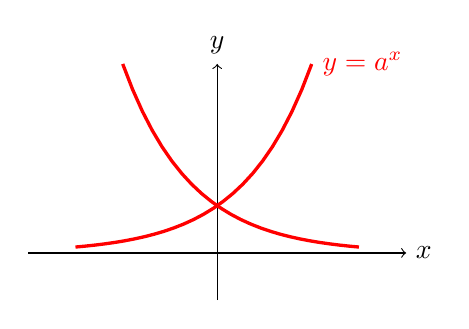
\begin{tikzpicture}[scale=0.6]
		\draw[->] (-4,0) -- (4,0) node[right] {$ x $};
		\draw[->] (0,-1) -- (0,4) node[above] {$ y $};
		\draw[very thick,color=red,domain=-3:2] plot (\x,{2 ^ \x}) node[right] {$ y = {a^x} $};
		\draw[very thick,color=red,domain=-2:3] plot (\x,{0.5 ^ \x});
	\end{tikzpicture}
	\caption{指数函数}
\end{figure}

\begin{tcolorbox}
	\mybox{指数函数}
	\begin{align}
		 & a^{-x} = {1 \over a^x}                    \\
		 & {1 \over a^{-x}} = a^x                    \\
		 & (ab)^x = a^xb^x                           \\
		 & ({a \over b})^x = {a^x \over b^x}         \\
		 & a^{kx} = (a^k)^x = (a^x)^k                \\
		 & a^ma^n = a^{m+n}                          \\
		 & {a^m \over a^n} = a^{m-n}                 \\
		 & a^{1/n} = \sqrt[n]{a}                     \\
		 & a^{m/n} = \sqrt[n]{a^m} = (\sqrt[n]{a})^m
	\end{align}
\end{tcolorbox}

\begin{tcolorbox}
	\mybox{Exercise}
	指数函数\\
	$ (6^{2k})^3 = 6^{6k} $\\
	$ 6^{k^2} \times 6 = 6^{k^2 + 1} $\\
	$ {3^k \over 9} = {3^k \over 3^2} = 3^{k-2} $\\
	$ 3^k \times 27 = 3^k \times 3^3 = 3^{k+3} $
\end{tcolorbox}

\vspace{0.5cm}

\subsection{对数函数(Logarithm Function)}

对于函数$ f: \{1,\ 2,\ 3,\ 4\} \rightarrow \{1,\ 4,\ 8,\ 16\},\ f(x) = 2^x $,指数函数是双射函数,因此它是有反函数的。\\

对数函数是指数函数的反函数,对数函数的定义为$ y = log_a{x}\ (a > 0\ |\ a \neq 1) $,其中$ a $称为底数。

\begin{figure}[H]
	\centering
	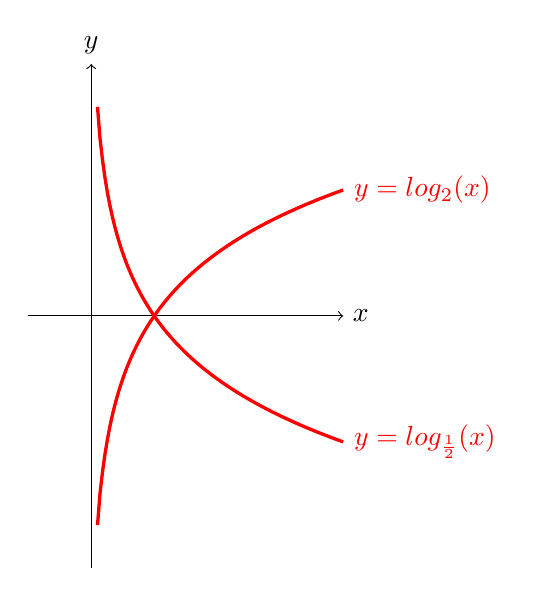
\begin{tikzpicture}[scale=0.8]
		\draw[->] (-1,0) -- (4,0) node[right] {$ x $};
		\draw[->] (0,-4) -- (0,4) node[above] {$ y $};
		\draw [very thick,color=red,domain=0.1:4,samples=100] plot (\x,{log2(\x)}) node[right] {$ y = log_2(x) $};
		\draw [very thick,color=red,domain=0.1:4,samples=100] plot (\x,{log10(\x) / log10(0.5)}) node[right] {$ y = log_{1 \over 2}(x) $};
	\end{tikzpicture}
	\caption{对数函数}
\end{figure}

\begin{tcolorbox}
	\mybox{对数函数}
	\begin{align}
		 & log_a(a^x) = x                                      \\
		 & a^{log_a(x)} = x                                    \\
		 & log_a(xy) = log_a(x) + log_a(y)                     \\
		 & log_a\left({x \over y}\right) = log_a(x) - log_a(y) \\
		 & log_a(x^n) = nlog_a(x)                              \\
		 & log_a(x) = {log_b(x) \over log_b(a)}
	\end{align}
\end{tcolorbox}

\begin{tcolorbox}
	\mybox{Exercise}
	对数函数\\
	$ log_5{k} + log_5{2} = log_5{2k} $\\
	$ log_2{5^2} = 2 \times log_2{5} $\\
	$ {log_3{k^2} \over log_3{25}} = {2 \times log_3{k} \over log_3{5^2}} = {2 \times log_3{k} \over 2 \times log_3{5}} = log_5{k} $
\end{tcolorbox}

\newpage